\section{Introduction}
\label{sec:intro}

\begin{figure*}[t]
\centering
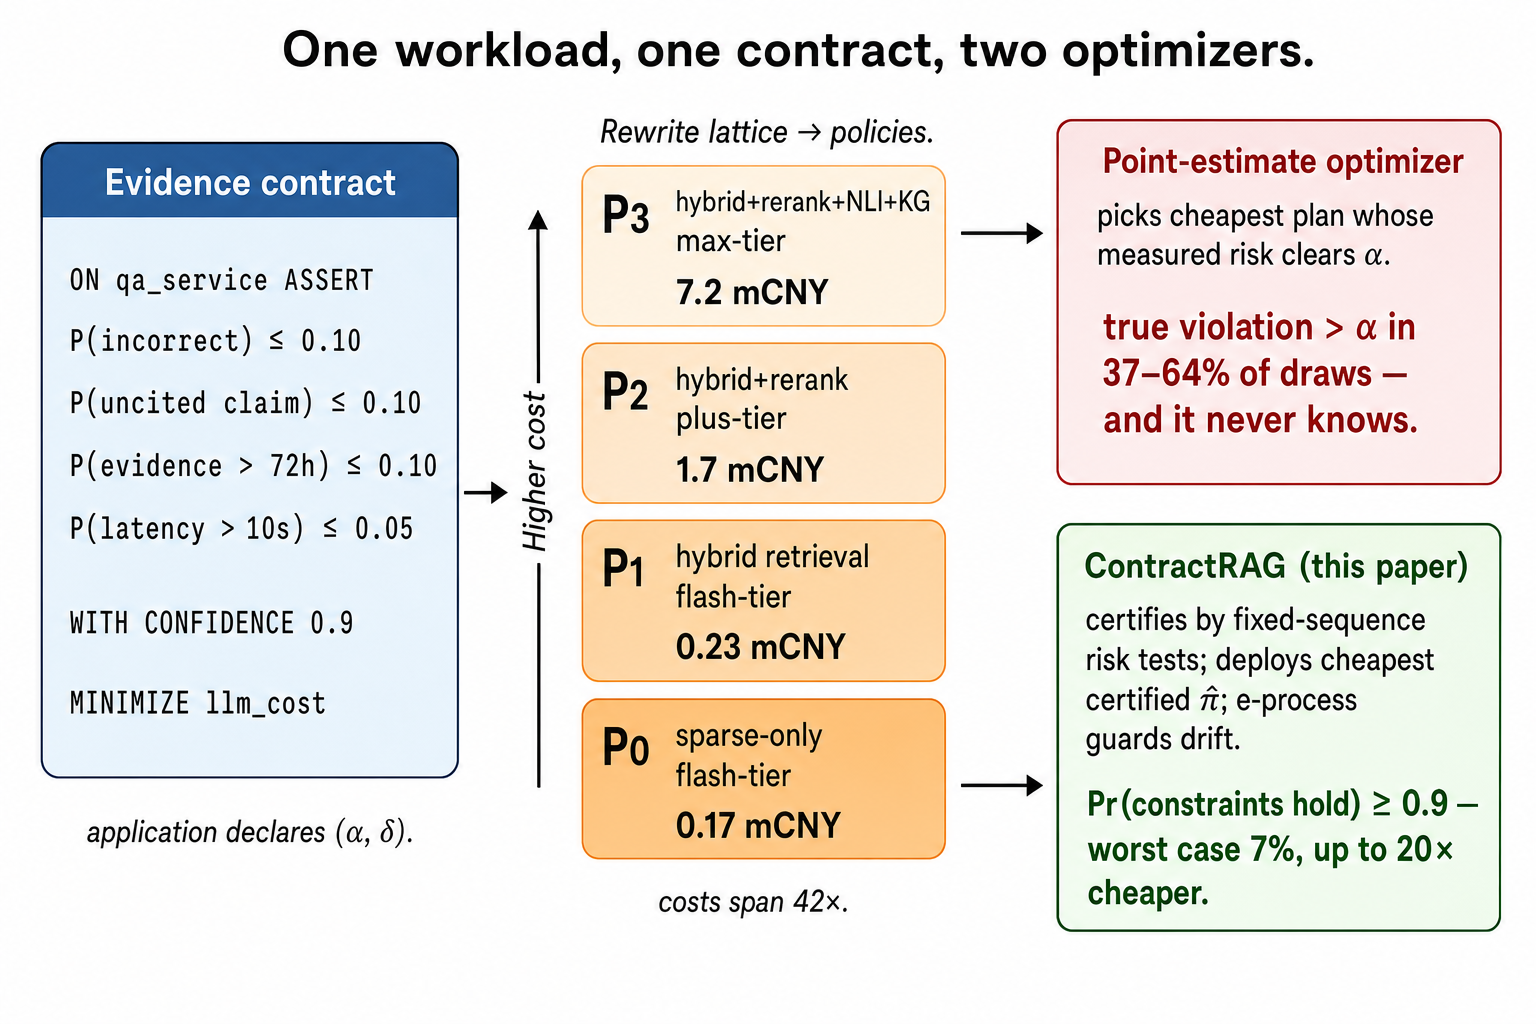
\includegraphics[width=\textwidth]{figures/fig_example_imagegen.png}
\caption{One workload, one contract, two optimizers. (Left) the
application declares admissible violation rates for correctness,
citations, freshness, and latency, plus a certification budget
$\delta=0.1$. (Center) cost-decreasing rewrites induce a space of plans
and per-query adaptive policies whose costs span 42$\times$. (Right) a
state-of-practice optimizer compares point estimates against the
constraint and routinely deploys infeasible plans; \system\ deploys the
cheapest policy that \emph{passes a statistical feasibility test}, so
the contract holds with probability $\ge 1-\delta$ for any query
distribution (Theorem~\ref{thm:validity}).}
\label{fig:example}
\end{figure*}


Retrieval-augmented generation (RAG) has quietly become a query
processing problem. Production question-answering services now span
relational tables, text corpora under sparse and dense indexes, vector
stores, and remote structured APIs; between retrieval and generation sit
fusion, reranking, verification, and a menu of LLMs whose per-token
prices span two orders of magnitude. Like a relational query, the same
information need admits many physical plans; unlike a relational query,
the plans do not return the same answer. A cheap plan answers most
queries correctly; an expensive plan answers more; no plan is correct
always. The defining question of RAG query optimization is therefore not
\emph{``which plan is equivalent and cheapest''} but \emph{``how much
answer risk may the application take, and what is the cheapest way to
stay within it?''}

\begin{example}
\label{ex:finance}
A brokerage deploys an assistant for questions such as \emph{``How did
Nvidia's data-center revenue last quarter compare to the consensus
estimate, and what did analysts say afterwards?''} A single answer joins
a finance API (fresh figures), crawled web pages (analyst commentary),
and tabular filings. Compliance imposes requirements on the
\emph{service}, not on any single answer: at most 10\% of answers may be
incorrect, at most 10\% may contain a claim without entailed citation or
cite evidence older than 72 hours, and at most 5\% may exceed a
10-second latency budget --- all at minimal LLM spend. The engineering team
can build a dozen pipelines that plausibly meet these requirements; what
they cannot do, with any tool available today, is \emph{know which ones
actually do} before violations reach customers.
\end{example}

Current systems answer this question with point estimates or not at all.
Workload-level optimizers for semantic operator pipelines --- Palimpzest,
LOTUS, DocETL, and most recently Abacus~\cite{russo2025abacus} --- sample
a handful of validation examples, estimate each plan's quality, and pick
the cheapest plan whose \emph{estimate} clears the target.
Adaptive-RAG-style routers~\cite{jeong2024adaptiverag} classify query
complexity and dispatch to pipelines with no feasibility statement
whatsoever. Conformal RAG methods~\cite{li2024traq,kang2024crag} do give
distribution-free guarantees, but for one fixed pipeline --- they neither
search a plan space nor reduce cost. The failure mode is structural, not
a matter of tuning: selecting the cheapest configuration whose
\emph{measured} risk clears a threshold is a multiple-testing procedure
without a correction, so the winner is systematically the plan whose
noise broke in its favor. We quantify this in \S\ref{sec:experiments}:
state-of-practice optimizers deploy policies whose true violation rate
exceeds the target in up to 64\% of calibration draws --- for the
brokerage of Example~\ref{ex:finance}, a coin flip on a compliance
requirement.

This paper proposes to make the promise a first-class object. An
\emph{evidence contract} declares admissible violation rates for answer
quality, citation completeness, evidence freshness, and latency,
together with a confidence budget $\delta$ for the certification itself.
\system, our optimizer, treats contract feasibility the way a database
treats integrity: no plan --- however attractive its point estimate ---
is deployable unless a statistical test on calibration executions
certifies it. Figure~\ref{fig:example} previews the interface and the
outcome on Example~\ref{ex:finance}'s workload. Three ideas make the
approach practical.

\textbf{Risk vouchers turn rewrites into a search space.} Classical
rewrites preserve semantics; RAG rewrites (retrieval truncation,
reranker elision, pre-filter pushdown, generator downgrade) trade
quality for cost by unknown amounts. \system\ annotates each rewrite
with an empirical \emph{risk voucher} --- a confidence upper bound on
its probability of harming an answer --- composes vouchers
assumption-free along rewrite chains by a telescoping argument, and
conditions them on estimated predicate selectivity, using the result
the way a classical optimizer uses a cost model: to order the
search, never to justify the result (\S\ref{sec:rewrites}).

\textbf{Certification survives search.} From the rewrite lattice
\system\ materializes per-query adaptive policies --- escalation ladders
driven by runtime sufficiency scores, cost-utility routers, and
group-conditional variants --- and walks them in a train-risk order with
fixed-sequence Hoeffding--Bentkus
tests~\cite{angelopoulos2021ltt,bentkus2004hoeffding}. The walk pays no
multiplicity penalty regardless of how many candidates are screened, so
enriching the policy space never erodes the guarantee
(\S\ref{sec:certification}).

\textbf{Monitoring closes the loop.} Certificates assume calibration
resembles deployment; hybrid RAG drifts --- workload mix shifts, indexes
fall behind, APIs degrade. An anytime-valid restart-mixture
e-detector~\cite{ramdas2023savi,shin2024edetectors} watches realized
violations with a change-time-independent detection-delay guarantee,
localizes the changepoint at $O(1)$ cost, and on alarm drives a
certified recalibration loop --- safe mode, post-alarm window,
fresh-budget recertification --- the statistical
descendant of mid-query re-optimization
\cite{kabra1998efficient,markl2004robust} (\S\ref{sec:monitor}).

The resulting guarantee is unconditional: for any query distribution,
any quality of the learned scores, and any candidate count, the deployed
policy satisfies all contract constraints with probability at least
$1-\delta$ (Theorem~\ref{thm:validity}). The learned components ---
sufficiency scorers, vouchers, orderings --- affect only how much money
the certified policy saves, never whether the contract holds. In this
division of labor, statistics plays the role of the execution engine and
machine learning the role of the cost model.

We evaluate on four tracks with fully metered execution: HybridQA
(tables + text), CRAG (web + knowledge-graph API,
with dynamism groups), and ALCE-ASQA and ALCE-QAMPARI (citation
contracts scored by the official TRUE-NLI evaluator). We verify the
guarantee directly on \emph{exact finite-population risk}: across
thirteen (track, $\alpha$) settings with 1000 repeated calibration
draws each, \system\ is the only method whose violation probability
stays below $\delta$ everywhere (worst case 0.8\%, an order of
magnitude inside the budget); empirical threshold tuning deploys truly
out-of-contract policies in up to 49\% of draws, and Bayesian
optimization, utility routing, and Abacus violate on most settings, in
up to 64\% of draws. At matched contract levels \system\ cuts cost
against the strongest fixed plan by 6.9$\times$ on HybridQA,
20$\times$ on CRAG, 15$\times$ on QAMPARI, and 1.4$\times$ on ASQA;
strict contracts down to $\alpha = 0.1$ certify once deferral to human
review is admitted --- and priced --- as a policy dimension; and its
group-conditional variant exposes --- and prices correctly --- the
up-to-19-point excess violation that marginal certification hides on
dynamic query slices. The guarantees and the savings are not artifacts
of one vendor's price sheet: swapping the generator ladder across four
model families from four developers --- DashScope-hosted Qwen,
DeepSeek, and GLM, and locally served Gemma~3 metered in GPU-seconds
--- certifies on every family, with savings up to 16.6$\times$ against
the family's strongest plan. A workload shift injected mid-stream is
detected by the e-process monitor in a median of 78 queries, with zero
false alarms across 200 drift-free control streams, the changepoint is
localized to within 4 queries, and a certified recalibration loop
restores the contract without oracle knowledge of the drift time ---
sustained across repeated alarms by geometric error spending, valid
under subsampled auditing, and with the audit spend itself metered
(20$\times$ becomes 10--18$\times$, honestly).

\smallskip\noindent\textbf{Contributions.}
\begin{itemize}
\item \emph{Evidence contracts} (\S\ref{sec:contracts}): a declarative,
statistically meaningful interface between RAG applications and the
execution engine, subsuming quality, citation, freshness, and latency
requirements.
\item \emph{Certified plan optimization} (\S\ref{sec:optimizer}): a
selection-proof optimizer combining rewrite-generated plan lattices,
assumption-free telescoping voucher composition,
selectivity-conditioned vouchers, cardinality-driven access-path
selection for the table$\bowtie$text join, and fixed-sequence testing
as the sole source of soundness --- with validity and cost-consistency
guarantees.
\item \emph{Certified progressive execution and monitoring}
(\S\ref{sec:runtime}): escalation policies whose stopping thresholds
carry the contract guarantee; group-conditional contracts; a
restart-mixture e-detector with a change-time-independent delay bound,
$O(1)$ changepoint localization, validity under subsampled audits, a
certified post-alarm recalibration loop, and a lifetime guarantee
across repeated alarms via geometric error spending.
\item \emph{Evaluation} (\S\ref{sec:experiments}): the first systematic
study of contract violation behavior across RAG optimizers on four
hybrid benchmarks --- verified on exact finite-population risk --- with
real metered cost across four model families from four developers on
two serving backends (token- and GPU-second-metered), plus voucher
coverage, strict contracts with deferral, four-constraint joint
contracts, drift detection with audit accounting, access-path,
plan-space-scale, and optimizer-overhead studies.
\end{itemize}
